\documentclass[12pt, a4paper, oneside]{ctexart}
\usepackage{amsmath, amsthm, amssymb, bm, color, graphicx, geometry, mathrsfs,extarrows, braket, booktabs, array, xcolor, fontspec, appendix, float, subfigure, wrapfig, enumitem}
\usepackage[colorlinks,linkcolor=red,anchorcolor=blue,citecolor=blue,urlcolor=blue,menucolor=black]{hyperref}

%%%% 设置中文字体 %%%%
\setCJKmainfont{方正新书宋_GBK.ttf}[BoldFont = 方正小标宋_GBK, ItalicFont = 方正楷体_GBK, BoldItalicFont = 方正粗楷简体]
%%%% 设置英文字体 %%%%
\setmainfont{Times New Roman}
\setsansfont{Calibri}
\setmonofont{Consolas}

%%%% 设置代码块 %%%%
% 在vscode中使用minted需要先配置python解释器, Ctrl+Shift+P, 输入Python: Select Interpreter选择安装了Pygments的Python版本. 再在setting.json中xelatex和pdflatex的参数中加入 "--shell-escape", 即可
% TeXworks中配置方法参考: https://blog.csdn.net/RobertChenGuangzhi/article/details/108140093
\usepackage{minted}
\renewcommand{\theFancyVerbLine}{
    \sffamily\textcolor[rgb]{0.5,0.5,0.5}{\scriptsize\arabic{FancyVerbLine}}} % 修改代码前序号大小
% 加入不同语言的代码块
\newmintinline{cpp}{fontsize=\small, linenos, breaklines, frame=lines}
\newminted{cpp}{fontsize=\small, linenos, breaklines, frame=lines}
\newmintedfile{cpp}{fontsize=\small, linenos, breaklines, frame=lines}
\newmintinline{matlab}{fontsize=\small, linenos, breaklines, frame=lines}
\newminted{matlab}{fontsize=\small, mathescape, linenos, breaklines, frame=lines}
\newmintedfile{matlab}{fontsize=\small, linenos, breaklines, frame=lines}
\newmintinline{python}{fontsize=\small, linenos, breaklines, frame=lines, python3}  % 使用\pythoninline{代码}
\newminted{python}{fontsize=\small, linenos, breaklines, frame=lines, python3}  % 使用\begin{pythoncode}代码\end{pythoncode}
\newmintedfile{python}{fontsize=\small, linenos, breaklines, frame=lines, python3}  % 使用\pythonfile{代码地址}

%%%% 设置行间距与页边距 %%%%
\linespread{1.2}
\geometry{left=2.5cm, right=2.5cm, top=2.5cm, bottom=2.5cm}

%%%% 定理类环境的定义 %%%%
\newtheorem{example}{例}            % 整体编号
\newtheorem{theorem}{定理}[section] % 定理按section编号
\newtheorem{definition}{定义}
\newtheorem{axiom}{公理}
\newtheorem{property}{性质}
\newtheorem{proposition}{命题}
\newtheorem{lemma}{引理}
\newtheorem{corollary}{推论}
\newtheorem{condition}{条件}
\newtheorem{conclusion}{结论}
\newtheorem{assumption}{假设}
\numberwithin{equation}{section}  % 公式按section编号 (公式右端的小括号)
\newtheorem{algorithm}{算法}

%%%% 自定义环境 %%%%
\newsavebox{\nameinfo}
\newenvironment{myTitle}[1]{
    \begin{center}
    {\zihao{-2}\bf #1\\}
    \zihao{-4}\it
}{\end{center}}  % \begin{myTitle}{标题内容}作者信息\end{myTitle}
\newcounter{problem}  % 问题序号计数器
\newenvironment{problem}[1][]{\stepcounter{problem}\par\noindent\textbf{题目\arabic{problem}. #1}}{\smallskip\par}
\newenvironment{solution}[1][]{\par\noindent\textbf{#1解答. }}{\smallskip\par}  % 可带一个参数表示题号\begin{solution}{题号}
\newenvironment{note}{\par\noindent\textbf{注记. }}{\smallskip\par}
\newenvironment{remark}{\begin{enumerate}[label=\textbf{注\arabic*.}]}{\end{enumerate}}
\BeforeBeginEnvironment{minted}{\vspace{-0.5cm}}  % 缩小minted环境距上文间距
\AfterEndEnvironment{minted}{\vspace{-0.2cm}}  % 缩小minted环境距下文间距


%%%% 图片相对路径 %%%%
\graphicspath{{figure/}} % 当前目录下的figure文件夹, {../figure/}则是父目录的figure文件夹
\setlength{\abovecaptionskip}{-0.2cm}  % 缩紧图片标题与图片之间的距离
\setlength{\belowcaptionskip}{0pt} 

%%%% 缩小item,enumerate,description两行间间距 %%%%
\setenumerate[1]{itemsep=0pt,partopsep=0pt,parsep=\parskip,topsep=5pt}
\setitemize[1]{itemsep=0pt,partopsep=0pt,parsep=\parskip,topsep=5pt}
\setdescription{itemsep=0pt,partopsep=0pt,parsep=\parskip,topsep=5pt}

\everymath{\displaystyle} % 默认全部行间公式, 想要变回行内公式使用\textstyle
\DeclareMathOperator*\uplim{\overline{lim}}     % 定义上极限 \uplim_{}
\DeclareMathOperator*\lowlim{\underline{lim}}   % 定义下极限 \lowlim_{}
\DeclareMathOperator*{\argmax}{arg\,max}  % 定义取最大值的参数 \argmax_{}
\DeclareMathOperator*{\argmin}{arg\,min}  % 定义取最小值的参数 \argmin_{}
\let\leq=\leqslant % 简写小于等于\leq (将全部leq变为leqslant)
\let\geq=\geqslant % 简写大于等于\geq (将全部geq变为geqslant)
\DeclareRobustCommand{\rchi}{{\mathpalette\irchi\relax}}
\newcommand{\irchi}[2]{\raisebox{\depth}{$#1\chi$}} % 使用\rchi将\chi居中

%%%% 一些宏定义 %%%%
\def\bd{\boldsymbol}        % 加粗(向量) boldsymbol
\def\disp{\displaystyle}    % 使用行间公式 displaystyle(默认)
\def\tsty{\textstyle}       % 使用行内公式 textstyle
\def\sign{\text{sign}}      % sign function
\def\wtd{\widetilde}        % 宽波浪线 widetilde
\def\R{\mathbb{R}}          % Real number
\def\N{\mathbb{N}}          % Natural number
\def\Z{\mathbb{Z}}          % Integer number
\def\Q{\mathbb{Q}}          % Rational number
\def\C{\mathbb{C}}          % Complex number
\def\K{\mathbb{K}}          % Number Field
\def\P{\mathbb{P}}          % Polynomial
\def\N{\mathbb{N}}          % Natural number
\def\Z{\mathbb{Z}}          % Integer number
\def\E{\mathbb{E}}          % Exception
\def\var{\text{Var}}        % Variance
\def\cov{\text{Cov}}        % Coefficient of Variation
\def\bias{\text{bias}}      % bias
\def\d{\mathrm{d}}          % differential operator
\def\e{\mathrm{e}}          % Euler's number
\def\i{\mathrm{i}}          % imaginary number
\def\re{\mathrm{Re}}        % Real part
\def\im{\mathrm{Im}}        % Imaginary part
\def\res{\mathrm{Res}}      % Residue
\def\D{\mathcal{D}}         % Dataset
\def\L{\mathcal{L}}         % Loss function
\def\O{\mathcal{O}}         % 时间复杂度
\def\wdh{\widehat}          % 宽帽子 widehat
\def\ol{\overline}          % 上横线 overline
\def\ul{\underline}         % 下横线 underline
\def\add{\vspace{1ex}}      % 增加行间距
\def\del{\vspace{-1.5ex}}   % 减少行间距

%%%% 正文开始 %%%%
\begin{document}
\begin{myTitle}{CVPR第五次作业-目标检测}
    强基数学\\
    吴天阳\quad 2204210460,马煜璇\quad 2204220461,申宇环\quad 2201422097,\\
    陈开来\quad 2205110920,王瑞恒\quad 2202113454
\end{myTitle}
\section{实验目的}
\begin{enumerate}
  \item 掌握HOG特征描述子和线性SVM分类算法.
  \item 理解滑动窗口进行目标检测方法.
  \item 掌握交并比(IoU)的原理与运用.
  \item 理解召回率、检验精度的概念,使用均值平均精度(mAP)评估目标检测器.
\end{enumerate}

具体方法:使用HOG特征和SVM设计单目标检测器.
\section{实验原理}
\subsection{方向梯度直方图(Hog)}
\subsubsection{图像预处理}
对原图像进行高斯模糊,降低噪声,利用Gamma校正公式对原图像亮度进行降低,$f(x) = x^{\gamma},\ (\gamma \geq 1)$,当$\gamma$越大时,图像亮度越低.
\subsubsection{梯度图计算}
使用Sobel算子分别计算$x$和$y$方向的偏导,两个方向上的偏导Sobel算子如下
\begin{equation*}
  W_x = \left[\begin{matrix}
    -1&0&1\\
    -2&0&2\\
    -1&0&1
  \end{matrix}\right],\quad W_y = \left[\begin{matrix}
    -1&-2&-1\\
    0&0&0\\
    1&2&1
  \end{matrix}\right]
\end{equation*}然后计算幅值(L2范数)和梯度方向:
\begin{equation*}
  g = \sqrt{g_x^2+g_y^2},\quad \theta = \left|\arctan\frac{g_y}{g_x}\right|
\end{equation*}
注:此处的梯度方向$\theta$是取过绝对值的结果,所以角度范围为$[0,\pi]$.
\subsubsection{梯度直方图计算}
由于梯度过于离散,对一个较大区域中全部梯度方向进行统计,首先假定cell大小为图像中$8\times 8$的一个区域,将原图划分为多个不交的$8\times 8$的区域,期望将$[0,\pi]$平均划分为$9$个部分(bins),然后将该区域中的梯度均摊到这$9$个辐角区间中来表示这个区域的辐角分布,如下$10$个端点构成的$9$个连续区间
\begin{equation*}
  \pi: 0,20^\circ, 40^\circ, 60^\circ, 80^\circ, 100^\circ, 120^\circ, 140^\circ, 160^\circ, 180^\circ
\end{equation*}
这也就是创建了大小为$9$的直方图数组,记为$h_1,\cdots,h_9$,然后该cell包含的每个像素点处的幅值按该像素点处的方向大小平均分配到最近的区间上即可.

举个例子,如果某像素点的幅值为$4$辐角为$65^\circ$,那么最近的两个区间点为$60^\circ, 80^\circ$对应数组为$h_4,h_5$,并且通过距离确定到两点的权重分别为$1/4,\ 3/4$,于是更新直方图数组为$h_4\rightarrow h_4+1/4\times 4,\ h_5\rightarrow h_5+3/4\times 4$.
\subsubsection{Block归一化}
计算出每个Cell的梯度直方图之后,再以$3\times 3$的cell作为一组,称为block. 由于每个cell包含$9$个值,所以一个block具有$3\times 3\times 9=81$个值,然后在通过滑动步长为$1$的block窗口,逐步输出每个位置的block值,最后拉成一个行向量,这就是\textbf{Hog特征},假设原图的大小为$40\times 100$,则cell个数为$5\times 12$,于是最终Hog特征维数为$(5-3+1)\times(12-3+1)\times 3\times 3\times 9 = 2430$.

再分析下每个block具体做些什么:一个block是由$3\times 3 = 9$个cell构成的,每个cell有$9$个变量,所以一共block存储的是$81$维向量,对齐进行归一化处理,就得到了该block所具有的信息.

\subsection{线性SVM模型}
在上述图像的Hog特征提取,得到了正例$550$个数据,负例$500$个数据,输入特征的维度为$2430$维,标签的只有正负两种. 所以我们可以使用SVM线性二分类器对数据进行分类,SVM的核心原理就是通过超平面对数据集进行划分,在数据集可分的情况下,使得正例全部在超平面的一侧,而负例在超平面的另一侧,如图\ref{fig-SVM}所示. 
\begin{figure}[htbp]
  \centering
  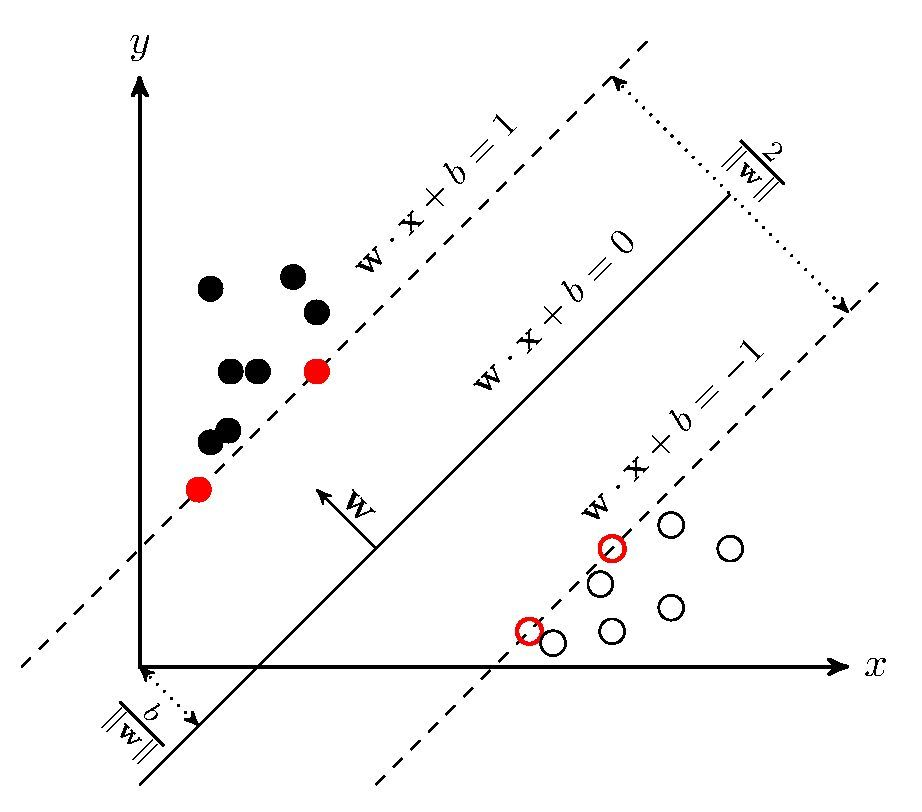
\includegraphics[scale=1]{SVM.jpg}
  \caption{SVM模型}
  \label{fig-SVM}
\end{figure}
假设样本的输入特征维数为$N$,则记特征向量为$\bd{x}\in \R^N$,特征$\bd{x}_i$对应的标签为$y_i$(正类记为$1$、负类记为$-1$),总训练数据为$M$个,数据集记为$\D = \{(\bd{x}_i, y_i):i=1,2,\cdots,M\}$. 

首先对特征向量拓展一个维度,新的维度中补$1$,这样就可以将超平面简化表达为$W'\bd{x}+b = W\bd{x}$,其中$W'\in\R^{1\times N},b\in\R,\ W\in\R^{1\times(N+1)}$.

设$d_i = y_i\frac{W\bd{x}_i}{||W||}$,则$d_i$表示第$i$个数据到超平面的矢量距离(若分类正确,则$d_i>0$否则$d_i<0$),则SVM的最优化问题为(最大化样本点到超平面的最小矢量距离):\del
\begin{align*}
  \max_{W}&\quad d = \min_{1\leq i\leq M}d_i,\\
  s.t.&\quad y_i\frac{W\bd{x_i}}{||W||}\geq d,\quad (i=1,2,\cdots, M)
\end{align*}
转化条件为$y_i\frac{W\bd{x}_i}{||W||d}\geq 1$,\add 如果我们记$\frac{W}{||W||d} = \bd{w}$,则最大化$d$,等价于最大化$||\bd{w}||^{-1}$,等价于最小化$\frac{1}{2}||\bd{w}||^2$,于是上述最优化问题进一步转化为\del
\begin{align*}
  \min_{\bd{w}}&\quad \frac{1}{2}||\bd{w}||^2,\\
  s.t.&\quad y_i\cdot\bd{w}\bd{x_i}\geq 1,\quad (i=1,2,\cdots, M)
\end{align*}
使用梯度下降法可对上述最优化问题进行优化,损失函数使用Hinge损失(合页损失)
\begin{equation*}
  L_i = \sum_{j\neq y_i}\max(0, s_j-s_{y_i}+1)
\end{equation*}

\subsection{目标检测}
\subsubsection{移动窗口检验}
对于一个任意大小的图像,我们考虑使用一个和图像相同大小的移动窗口(保持提取的特征之前Hog特征提取的维度相同),由于图像中的目标大小不一定保持大小相同,我们期望使用Gauss金字塔对原图进行缩放(这里主要做图像缩小),主要原理就是使用Gauss核进行下采样. 然后在缩小后的图像上进行窗口平移,对每个窗口的Hog特征提取出来,然后利用已搭建的SVM模型进行预测,从而得到每个窗口图像的置信度. 最终将置信度最高的一组图像进行输出即可.
\subsubsection{loU非最大值抑制}
在不同的Gauss金字塔图像中,我们获得了不同大小的检测框,此时检测框可能有较大的重叠,需要从重叠率较高的检测框中选取其中置信度最高的一个作为输出,这里引入交并比(Intersection over Union, IoU)作为检测框重叠率的评判标注.

假设$A,B$表示两个检测框,记面积函数$S(\cdot)$用于计算区域的面积,则$A$与$B$的交并比为(第二个等号利用容斥原理)
\begin{equation*}
  \text{IoU}(A,B) = \frac{S(A\cap B)}{S(A\cup B)} = \frac{S(A\cap B)}{S(A)+S(B)-S(A\cap B)}
\end{equation*}
在实际计算中往往使用容斥原理计算$S(A\cup B)$.

定义重叠阈值$\lambda$,若检测框$A,B$的IoU值大于$\lambda$,则认为$A,B$重叠,将两者中置信度高的保留下来,一次反复,最终保证留下的检测框两两不重叠. 具体实现中,可以先对置信度进行排序,将置信度最高的检测框保留,然后将置信度低的与已保留的检测框进行比对,判断是否有重叠,若重叠则直接舍去,反之保留.

\subsection{评估目标检测器}
使用mAP(mean Average Precision)值对目标检测器进行评估首先引入AP(Average Precision)值,即\textbf{精度与召回率曲线围成的平均面积},首先进行如下几个定义:
\begin{enumerate}
  \item \textbf{True Positive(TP)}:检测框与真实框的IoU比值大于阈值(一般为$0.5$,同一真实框只计算一次)的数量.
  \item \textbf{False Positive(FP)}:检测框与真实框的IoU比值小于阈值或重复检测真实框的数量.
  \item \textbf{False Negative(FN)}:未被检测到的额真实框数量.
  \item \textbf{精度(Precision)}:检测到的检测框占当前总检测框的比值$P = \frac{TP}{TP + FP}$.\add
  \item \textbf{召回率(Recall)}:检测到的真实框占总真实框的比值$R = \frac{TP}{TP + FN}$.
\end{enumerate}

计算AP曲线首先要计算PR曲线,过程主要分为以下几步:
\begin{enumerate}
  \item 对一幅图像中全部检测框按照置信度从高到低排序.
  \item 选取当前置信度最高的检测框,若该检测框能匹配到真实框,则$TP+1$,否则$FP+1$.
  \item 在PR曲线上,当前框的绘制$(P,R)$点.
  \item 若仍有剩余检测框,则回到第$1$步. 否则循环.
\end{enumerate}
通过上述方法可以得到PR曲线图,图上绘制点的个数为检测框总数目. 由于PR曲线图不够平滑,我们将每个Recall点的$P$值重新计算,以右侧最大的$P$值作为代替值(这也是一种插值),即$P_{interp}(r) = \max_{r' > r}P(r')$,如图\ref{fig-interp}所示
\begin{figure}[htbp]
  \centering
  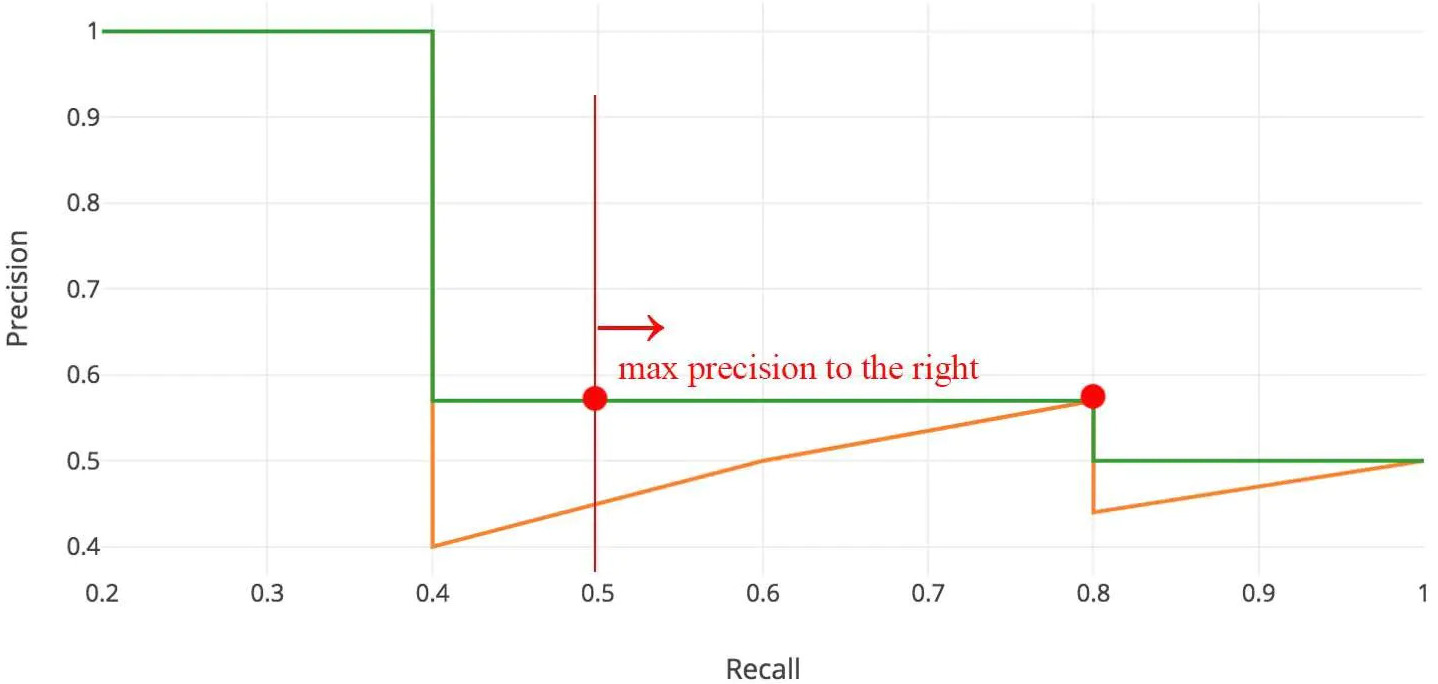
\includegraphics[scale=1]{interp.jpg}
  \caption{AP曲线插值方法}
  \label{fig-interp}
\end{figure}
在计算插值后得到AP曲线与$x$轴围成的面积即为该种类别的\textbf{AP值}.

设总图像类别有$K$种,记第$i$中类别的AP值为$AP_i$,则该分类器的$mAP$值为
\begin{equation*}
mAP = \frac{\sum_{i=1}^K AP_i}{K}
\end{equation*}

一个目标检测模型的mAP值越高说明该型的性能越好.

\section{实验步骤与结果分析}
本次代码难度较大,参考老师教程使用GitHub中项目完成. 特征提取及SVM模型训练:\href{https://github.com/bikz05/object-detector/tree/master/object-detector}{GitHub-bikz05/object-detector},mAP评价目标检测器:\href{https://github.com/Cartucho/mAP}{Cartucho/mAP}
\subsection{计算Hog特征}
首先利用\pythoninline{extract-features.py}进行Hog特征提取,使用\pythoninline{skimage.feature.hog}对目标进行提取,正例图像处理的核心代码如下(处理反例只需将文件路径修改即可):
\begin{pythoncode}
for im_path in glob.glob(os.path.join(pos_im_path, "*")):  # 读取图片路径
    im = cv2.imread(im_path, cv2.IMREAD_GRAYSCALE)  # 灰度图像读入
    fd = feature.hog(im, orientations=9,  # 将角度分为9个区间
                      pixels_per_cell=(8, 8),  # cell大小
                      cells_per_block=(3, 3))  # block大小
    fd_name = os.path.split(im_path)[1].split(".")[0] + ".feat"
    fd_path = os.path.join(pos_feat_ph, fd_name)  # 设置保存文件路径
    joblib.dump(fd, fd_path)  # 保存图像的Hog特征
\end{pythoncode}

图\ref{fig-hog}是我们自己尝试Hog特征提取结果:
\begin{figure}[htbp]
  \hspace*{-1.1cm}
  \centering
  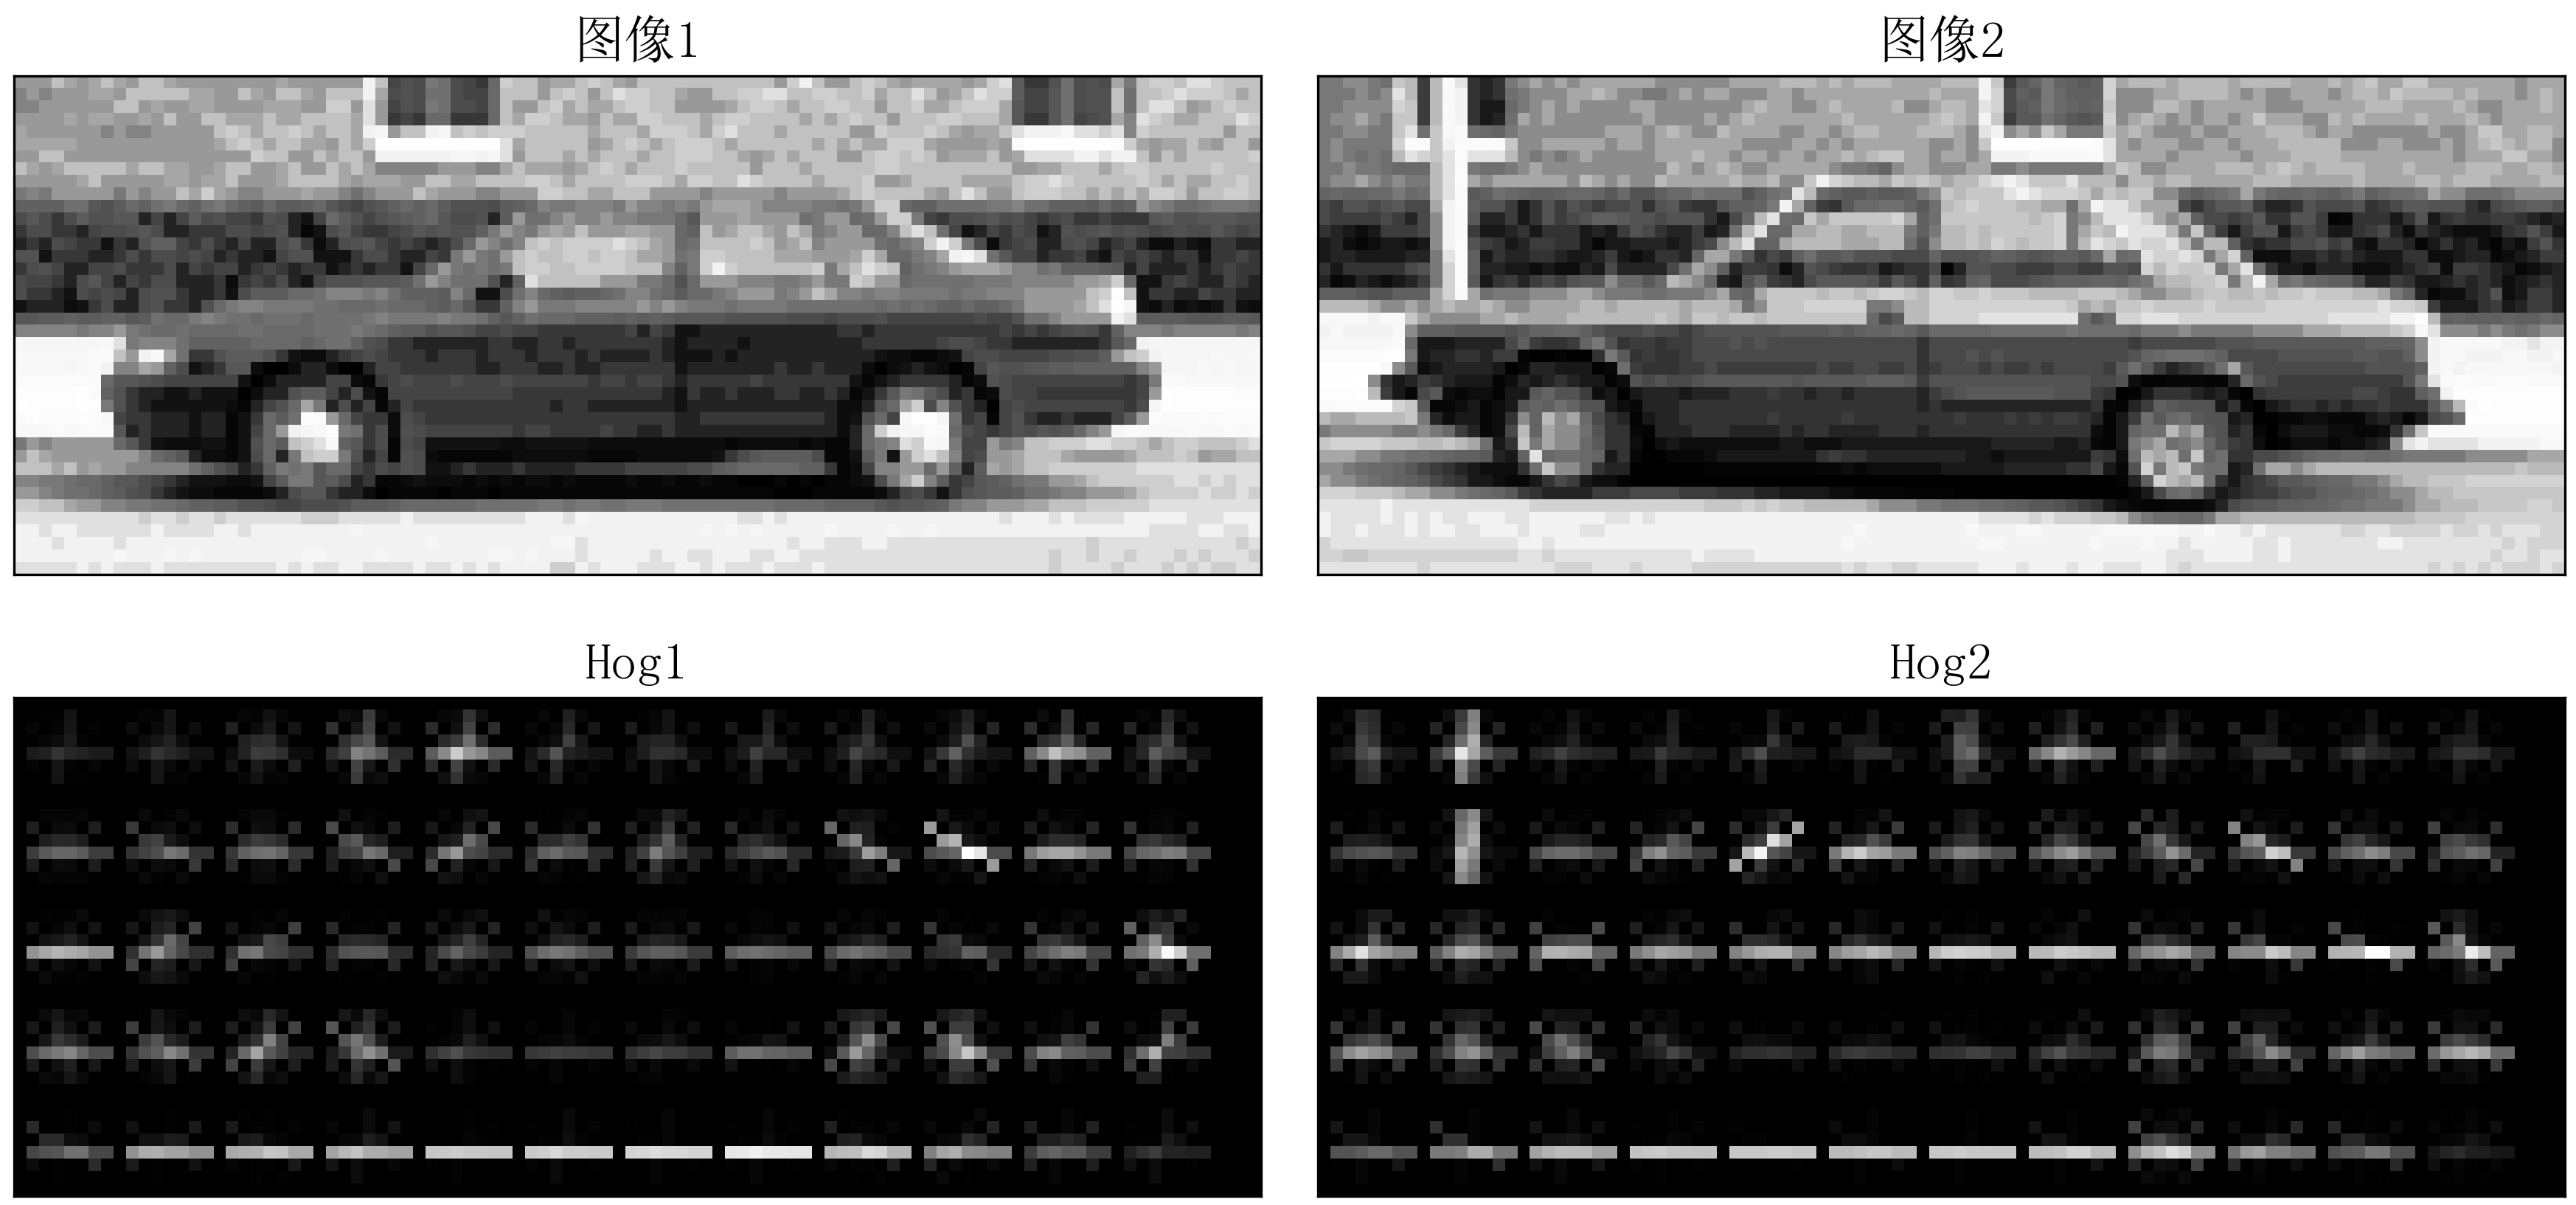
\includegraphics[scale=0.6]{hog特征提取.png}
  \caption{Hog特征提取}
  \label{fig-hog}
\end{figure}
\subsection{SVM模型训练}
利用\pythoninline{train-classifier.py}搭建SVM二分类模型,并使用上述Hog特征对模型进行训练
\begin{pythoncode}
from sklearn.svm import LinearSVC, SVC  # 使用sklearn的SMV模型

clf = LinearSVC()  # 初始化SVM模型
clf.fit(fds, labels)  # Hog特征及对应的标签进行训练
joblib.dump(clf, model_path)  # 保存模型
\end{pythoncode}
\subsection{目标检测}
使用\pythoninline{test-classifier.py}实现对任意图像的目标检测,同时输出检测过程和经过NMS处理交并比后的检测框,通过阅读源码学习到了以下技巧:
\begin{pythoncode}
# 利用迭代器的形式返回滑动窗口的图像(可简化主函数中的for循环)
def sliding_window(image, window_size, step_size):
    for y in range(0, image.shape[0], step_size[1]):
        for x in range(0, image.shape[1], step_size[0]):
            yield x, y, image[y:y+window_size[1], x:x+window_size[0]]

    # Gauss金字塔使用1.25倍做小比例
    for im_scaled in pyramid_gaussian(im, downscale=downscale):
        # 如果图像大小小于检测窗口大小,跳过
        if im_scaled.shape[0] < min_wdw_sz[1] or im_scaled.shape[1] < min_wdw_sz[0]:
            break
        # 此处使用迭代器函数,简化for函数,增强可读性
        for (x, y, im_window) in sliding_window(im_scaled, min_wdw_sz, step_size):
            # 如果窗口大小小于检测窗口大小,跳过
            if im_window.shape[0] != min_wdw_sz[1] or im_window.shape[1] != min_wdw_sz[0]:
                continue
            # 对窗口进行Hog特征提取
            fd = feature.hog(im_window, orientations=9, pixels_per_cell=(8, 8), cells_per_block=(3, 3), visualize=False)
            fd_reshape = fd.reshape(1, -1)
            # 使用SVM进行预测
            pred = clf.predict(fd_reshape)
        if pred == 1:  # 若预测为真
            ... # 保存两种比例的检测框,一个为当且缩放后的图像,另一个还原回原始图像(增大downscale的幂次倍)
\end{pythoncode}
我们对滑动窗口可视化部分的代码重新实现了一遍,主要使用了\pythoninline{cv2.rectangle(im, (y0, x0), (y1, x1), (R,G,B), thickness=2)},表示在图像\pythoninline{im}上绘制处位于左上角坐标为\pythoninline{(y0, x0)}右下角坐标为\pythoninline{(y1, x1)}粗细为\pythoninline{thickness}的颜色为\pythoninline{(B,G,R)}的矩形边框. 窗口移动的方法是通过反复在同一张图像上进行绘制,并设置每帧图像显示时长,利用api函数\pythoninline{cv2.waitKey(x)}显示\pythoninline{x}毫秒控制每帧时长,从而实现动画效果. 代码如下,由于动画效果不宜展示,所以选取了几个静态的窗口位置,如图\ref{fig-rectangle}所示.
\begin{pythoncode}
# Gauss金字塔的基础上做滑动窗口
for i, im_scaled in enumerate(transform.pyramid_gaussian(im, downscale=downscale, channel_axis=-1)):
    for x, y, im_window in sliding_window(im_scaled, (30, 100), (30, 30)):
        if im_window.shape[0] != 30 or im_window.shape[1] != 100:
            continue
        clone = im_scaled.copy()  # 在原图上重新绘制
        cv2.rectangle(clone, (y, x), (y + 100, x + 30), (255,255,255), thickness=2)  # 绘制窗口
        cv2.imshow("Sliding Window", clone)  # 显示窗口
        cv2.waitKey(100)  # 控制每帧长度
\end{pythoncode}
\begin{figure}[htbp]
  \centering
  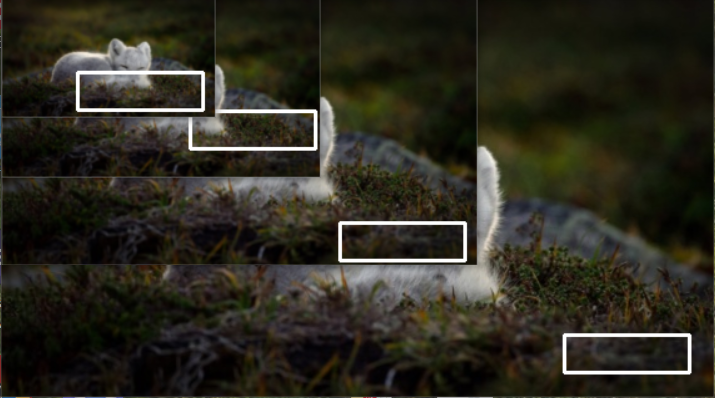
\includegraphics[scale=0.5]{Gauss_Sliding.png}
  \caption{Gauss金字塔基础上的滑动窗口}
  \label{fig-rectangle}
\end{figure}
通过IoU非最大值抑制可以将多个重叠框中置信度最高的一个选出来,具体做法如下:
\begin{pythoncode}
def overlapping_area(detection_1, detection_2):  # 计算交并补
    x1_tl = detection_1[0]  # 左端点
    x2_tl = detection_2[0]
    x1_br = detection_1[0] + detection_1[3]  # 右端点
    x2_br = detection_2[0] + detection_2[3]
    y1_tl = detection_1[1]  # 上端点
    y2_tl = detection_2[1]
    y1_br = detection_1[1] + detection_1[4]  # 下端点
    y2_br = detection_2[1] + detection_2[4]
    # 交集区域,右下端点取min,左上端点取max,即可得到交集区域
    x_overlap = max(0, min(x1_br, x2_br)-max(x1_tl, x2_tl))
    y_overlap = max(0, min(y1_br, y2_br)-max(y1_tl, y2_tl))
    overlap_area = x_overlap * y_overlap
    area_1 = detection_1[3] * detection_2[4]
    area_2 = detection_2[3] * detection_2[4]
    # 利用容斥原理计算并集区域
    total_area = area_1 + area_2 - overlap_area
    return overlap_area / float(total_area)

def nms(detections, threshold=.5):
    if len(detections) == 0:
        return
    # 首先基于置信度从高到低排序
    detections = sorted(detections, key=lambda detections: detections[2], reverse=True)
    new_detections=[]  # 保存最终选取的检测框
    new_detections.append(detections[0])
    del detections[0]  # 加入第一个检测框,并从检测框序列中删除
    for index, detection in enumerate(detections):
        # 每次从剩余的检测框中选出置信度最高的
        for new_detection in new_detections:
        # 若和已保存检测框重叠,说明该检测框与置信度更高的检测框重叠,故将其删去
            if overlapping_area(detection, new_detection) > threshold:
                del detections[index]
                break
        else:  # 若无检测框重叠则保存检测框,使用for/else语法,非常巧妙
            new_detections.append(detection)
            del detections[index]
    return new_detections
\end{pythoncode}
最终目标检测效果如图\ref{fig-detections}所示(上排图像从右到左为Gauss金字塔从大到小生成的结果,红框为滑动窗口过程中检测到的结果,左下角为全部过程中检测结果,右下角蓝框为nms处理重叠后的结果)
\begin{figure}[htbp]
  \centering
  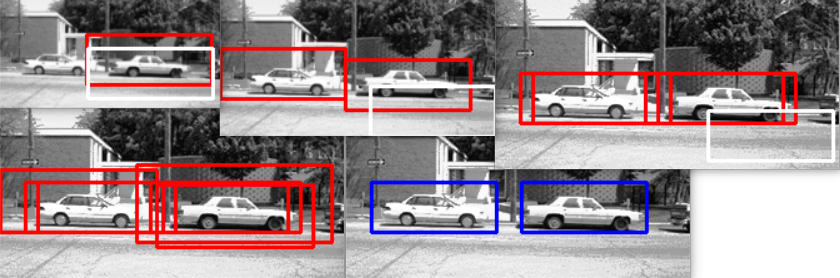
\includegraphics[scale=0.5]{detections.png}
  \caption{目标检测结果}
  \label{fig-detections}
\end{figure}
\subsection{评估目标检测器}
首先利用\pythoninline{test-clf-full.py}将测试集中每张图像预测的检测框保存为\pythoninline{.txt}文件格式,这里用到一个快捷保存到\pythoninline{.txt}文件的api函数\pythoninline{np.savetxt(fname, output, fmt='%s')}:表示将output转化为\pythoninline{np.ndarray}格式后,输出到\pythoninline{fname}文件中(以空格作为默认分隔符).

注:由于需要转化为矩阵的形式,所以必须保证每行的列数目相同. 例如:
\begin{pythoncode}
a = np.arange(6).reshape(-1, 3)
output = [('test1', '123', '321'), ('test2', '456', 654), *a.tolist()]
np.savetxt('test.txt', output, fmt='%s')
''' text.txt中内容
test1 123 321
test2 456 654
0 1 2
3 4 5
'''
\end{pythoncode}

使用\pythoninline{convert_gt_txt.py}将数据集中人工标定的真实框结果转化为指定格式,便于后续比较.

在使用\pythoninline{intersect-gt-and-dr.py}将真实框数目和检测框数目保持一致,这里总共有170个真实框,而检测框只有163个,说明有7个图像没有检测到任何车辆.

最后使用\pythoninline{evaluate-mAP.py}实现mAP计算,最终得到的结果为$92.84\%$.
\begin{figure}[htbp]
  \centering
  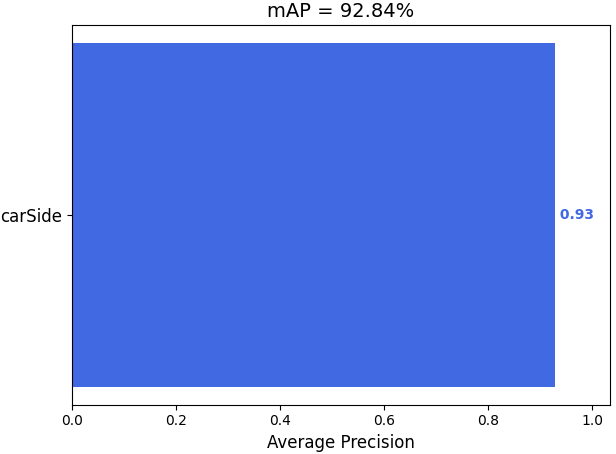
\includegraphics[scale=0.6]{mAP.png}
  \caption{mAP}
\end{figure}
\section{结论与讨论}
通过本次实验,我们学习到了基本的目标检测方法,通过阅读源代码,学习到了很多有用的技巧,在复杂项目中安排代码结构,当代码具有多种输入参数时,可以使用\pythoninline{argparse}库来解析cmd中输入的命令参数,便于调用代码,无需在IDE中打开后依次执行,或者使用脚本一次性运行整个项目的代码. 还学习到如何利用\pythoninline{opencv}绘制动态检测框效果,可以为以后自己实现这类问题提供思路.
\end{document}